\chapter{Theoretische Grundlagen}

Die additive Fertigung hat in den letzten Jahren Fortschritte gemacht und ist zu einem Bestandteil der modernen Fertigungstechnologie geworden. Innerhalb dieses Prozesses werden Bauteile über CAD \texttt{(computer aided design)} entworfen. Über Verfahren der additiven Fertigung werden diese Bauteile dann gefertigt. FDM-Druck hat sich als eine vielversprechende Methode etabliert, um komplexe dreidimensionale Objekte schichtweise aufzubauen. Während FDM-Druckverfahren traditionell auf Polymermaterialien ausgerichtet sind, hat die Weiterentwicklung dieser Technologie nun den Weg für den Einsatz von Metallfilamenten eröffnet. In diesem Kapitel werden die theoretischen Grundlagen erläutert.

\subsection{Additive Fertigung und der FDM-Prozess}

Additive Fertigung wird als Verfahren bezeichnet, bei dem Materialien entweder durch Verschmelzung, Bindung oder Verfestigung von Materialien wie flüssigen Harzen und Pulvern gemischt werden. Im Gegensatz dazu stehen subtraktive Verfahren, die einen Abtrag von Material hervorrufen, wie zum Beispiel CNC \texttt{(Computer Numerical Control)}. Bei additiven Verfahren wird das zuvor entwickelte 3D-Bauteil in einzelne Schichten unterteilt um die gewünschte Geometrie zu erreichen. Diese Schichten werden aus einer STL-Datei gemeriert, dazu wird eine spezielle Software verwendet um alle Einstellungen zu treffen. Hier ist auch ein essentieller Unterschied zur \texttt{CNC-}Fertigung, denn mithilfe dieser Software wird unter anderem die Auflösung des Bauteils vorgegeben, welches unter anderem Einflüsse auf die Fertigungszeit hat.\\
Der Begriff FDM  \texttt{(Fused Deposit Modeling)} wurde 1989 zuerst erwähnt und beschreibt das Prinzip bei dem Rohmaterial durch einer aufgeheizten Düse extrudiert wird. Die Extrusion wird auf ein spezielles Druckbett appliziert. Die Extrusion bildet Linien, welche dann aneinander gereit eine Schicht ergibt.

\autocite{Osama2019}

\subsection{Materialien für den FDM-Prozess}

Bisher werden meistens verschiedenste Kunststoffe, oder eine Mischung derer, für den FDM-Druck verwendet.

\subsection{316L-Edelstahl als Druckmaterial}

Obwohl der FDM-Druck vorwiegend für Kunststoffe verwendet wird, haben viele Firmen mit der Entwicklung von Metallfilamenten begonnen. Diese Filamente binden Metallpartikel in einem Polymer. Anders als beim SLM \texttt{Selective Laser Melting}, bei dem Metallpartikel mittels eines Lasers aufgeschmolzen wird, entstehen somit kein gefährlicher, aufgewirbelter Staub. \autocite{MetalAdditiveMan}
\begin{figure}[h]
	\centering
	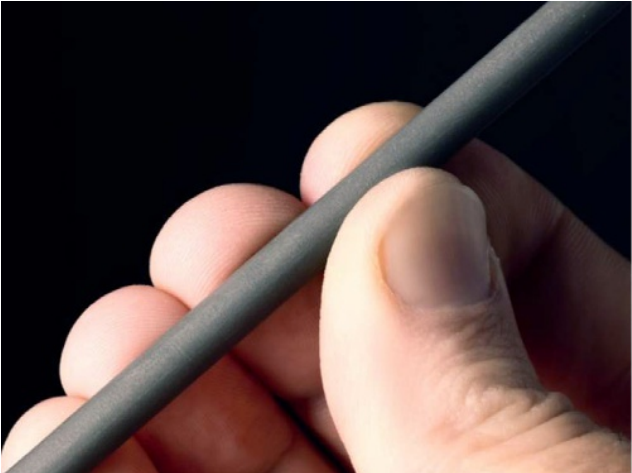
\includegraphics[width=0.5\linewidth]{bilder/Beispiel_Metallfilament.png}
        \caption[Beispiel für ein Metallfilament in Rohform] {Beispiel für ein Metallfilament in Rohform \autocite{MetalAdditiveMan}}
	\label{fig:FilamentBeispiel}
\end{figure}

Nachdem die gewünschte Kontur gefertigt ist, besteht sie weiterhin aus Metallpartikel gebunden mit Polymer. Damit dieses Polymer nun entweicht, wird es entbunden. Dazu wird das Bauteil in ein Bad aus Lösemittel für eine bestimmte Zeit gegeben. Dadurch löst sich das Polymer größtenteils und verlässt die Struktur. Übrig bleibt die Metallpartikel in der Geometrie. Zuletzt wird das Bauteil in eine Sinteranlage gegeben. Dort wird es auf bis zu 1400C° erhitzt in Wasserstoffumgebung. Hierbei wird eine bestimmte Temperaturkurve mit Aufheiz-, Halte- und Abkühlphasen.\\
Dadurch verbinden sich die Metallpartikel auf molekularer Ebene und das fertige Metallteil ist fertig. Zu beachten ist jedoch, dass das Volumen durch den Entbinder- und Sinterprozess schwindet, da das Polymer gelöst wird.

\subsection{Dichte- und Schwindungsbegriffe}